%%
%% Copyright 2007, 2008, 2009 Elsevier Ltd
%%
%% This file is part of the 'Elsarticle Bundle'.
%% ---------------------------------------------
%%
%% It may be distributed under the conditions of the LaTeX Project Public
%% License, either version 1.2 of this license or (at your option) any
%% later version.  The latest version of this license is in
%%    http://www.latex-project.org/lppl.txt
%% and version 1.2 or later is part of all distributions of LaTeX
%% version 1999/12/01 or later.
%%
%% The list of all files belonging to the 'Elsarticle Bundle' is
%% given in the file `manifest.txt'.
%%

%% Template article for Elsevier's document class `elsarticle'
%% with numbered style bibliographic references
%% SP 2008/03/01
%%
%%
%%
%% $Id: elsarticle-template-num.tex 4 2009-10-24 08:22:58Z rishi $
%%
%%
\documentclass[preprint,review,10pt,3p]{elsarticle}

%% Use the option review to obtain double line spacing
%% \documentclass[preprint,review,12pt]{elsarticle}

%% Use the options 1p,twocolumn; 3p; 3p,twocolumn; 5p; or 5p,twocolumn
%% for a journal layout:
%% \documentclass[final,1p,times]{elsarticle}
%% \documentclass[final,1p,times,twocolumn]{elsarticle}
%% \documentclass[final,3p,times]{elsarticle}
%% \documentclass[final,3p,times,twocolumn]{elsarticle}
%% \documentclass[final,5p,times]{elsarticle}
%% \documentclass[final,5p,times,twocolumn]{elsarticle}

%% if you use PostScript figures in your article
%% use the graphics package for simple commands
%% \usepackage{graphics}
%% or use the graphicx package for more complicated commands
\usepackage{graphicx}
%% or use the epsfig package if you prefer to use the old commands
%% \usepackage{epsfig}

\usepackage{subfigure}
\usepackage[linesnumbered,ruled, boxed]{algorithm2e}

%% The amssymb package provides various useful mathematical symbols
\usepackage{amssymb}
%% The amsthm package provides extended theorem environments
%% \usepackage{amsthm}

%% The lineno packages adds line numbers. Start line numbering with
%% \begin{linenumbers}, end it with \end{linenumbers}. Or switch it on
%% for the whole article with \linenumbers after \end{frontmatter}.
%% \usepackage{lineno}

%% natbib.sty is loaded by default. However, natbib options can be
%% provided with \biboptions{...} command. Following options are
%% valid:

%%   round  -  round parentheses are used (default)
%%   square -  square brackets are used   [option]
%%   curly  -  curly braces are used      {option}
%%   angle  -  angle brackets are used    <option>
%%   semicolon  -  multiple citations separated by semi-colon
%%   colon  - same as semicolon, an earlier confusion
%%   comma  -  separated by comma
%%   numbers-  selects numerical citations
%%   super  -  numerical citations as superscripts
%%   sort   -  sorts multiple citations according to order in ref. list
%%   sort&compress   -  like sort, but also compresses numerical citations
%%   compress - compresses without sorting
%%
%% \biboptions{comma,round}

% \biboptions{}

\usepackage[utf8]{inputenc}



\usepackage{todonotes}
\newcommand{\todop}[1]{\todo{P: #1}}


\journal{IPL}


\begin{document}

\begin{frontmatter}


%\mainmatter  % start of an individual contribution

% first the title is needed
\title{Gradient Boosting to Fuse Multiple Sources of Relevance Evidence in Search Indexes}

\author[mymainaddress]{Sheila N{\'obrega}}
\author[mymainaddress]{Edleno Moura}
\author[mysecondaryaddress]{P{\'a}vel Calado}
\author[mymainaddress]{Altigran Silva}

\address[mymainaddress]{Universidade Federal do Amazonas, Brasil}
\address[mysecondaryaddress]{INESC-ID, Instituto Superior T{\'e}cnico, Universidade de Lisboa}

\begin{abstract}

In this paper we address the problem of using a learning to rank technique to fuse sources of relevance evidence at indexing time in search systems. We propose a modified Gradient Boosted Regression Tree algorithm to generate \textit{unified term impacts} (UTI) to be stored in the index.
The UTI is the only value needed later for ranking the documents, thus greatly reducing the effort needed to compute the document scores. 
Our approach achieves better results in quality, when compared to previously proposed methods to compute UTI, while requiring much less time for training. In addition, we show how to obtain significant gains in index compression with virtually no loss in the quality of search results.

\begin{keyword}
\texttt Learning to Rank \sep Search Engines \sep Indexing \sep LambdaMART \sep Gradient Boosting
\end{keyword}

\end{abstract}
\end{frontmatter}


%%
%% Start line numbering here if you want
%%
% \linenumbers

%% main text

\section{Introduction}
\label{intro}

The production of high quality ranking results is a fundamental aspect of Web search engines. Users expect the answers to their queries to be shown at the top of the list and rarely go beyond the first page displayed~\cite{saraiva2001rank}. 

Further, modern search engine users are used to experience fast query processing times, regardless of the size of the dataset, and any noticeable increase in waiting time can be a fatal blow to the their perception of the quality of the system. Thus,
computational efficiency cannot be obtained at the cost of quality. 

The issue of quality is usually addressed through a class of machine learning techniques commonly known as \textit{learning to rank} (L2R). Query processing by a L2R-based search engine is performed in two steps: first, the top-k documents for a query are retrieved using a low cost ranking strategy, such as BM25, referred to as \emph{base ranker}; second, the documents are re-ranked with the more expensive L2R model, referred to as \emph{top-ranker}~\cite{capannini2016quality}.

An important aspect of modern search engines is the use of a large number of distinct sources of \emph{relevance evidence} to build the L2R model. Collectively, these determine whether or not the document is relevant to a query. Examples of such sources of relevance evidence are the frequencies of terms in the text, urls, titles and other parts of the document, web link graph analysis, among others~\cite{baezaribeiro2011modinforet}. 

The ranking of query results is computed by fusing all sources of evidence into a single document score, for each document in the final ranking. In the past few decades, most work on fusing evidence has been done with the deployment of L2R methods~\cite{liu11:L2RfIR}.

L2R methods use examples of queries and their respective results, to train supervised learning models that determine the relative position of the documents in the result list. Once trained, the model can be used during query processing to determine the final ranking. This approach, however, inadvertently adds computational costs to query processing, which may lead to a drop in time performance.

\newcommand{\lepref}{LePrEF}
\newcommand{\lambdamart}{LambdaMART}

To mitigate this problem, an alternative approach has been proposed --- Learn to Precompute Evidence Fusion (\lepref)~\cite{costa2012lepref}, also based on supervised learning techniques. \lepref\ proposes to implement the bulk of the evidence fusion during indexing time, generating a single inverted index containing unified entries representing all sources of evidence. These unified entries are called \textit{Unified Term Impacts} (UTIs). 

Each UTI is computed based on a pre-trained L2R model and, at query time, the search engine needs only to sum each of the query term's UTI to directly obtain the document scores.

In this work, we propose and study an adaptation of \lambdamart~\cite{wu2010lambdamart}, a gradient boosting algorithm, to compute the UTIs of each term at indexing time.
We improve the work done on \lepref\ in two ways. First, we significantly reduce the required training time, while by carefully tuning the algorithm, we still achieve high quality search results. Second, using a simple compression procedure, we are able to greatly reduce the space requirements of the inverted index, without significant loss in search quality. 

In the remainder of this text, we refer to our approach as UTI-LambdaMART. We present experiments to compare the performance of UTI-LambdaMART with the work of~\cite{costa2012lepref},
%UTI using GP 
where our adaptation of \lambdamart\ achieves results in 2.8\% of the time required by \lepref %using GP 
without loss of quality. Further, the use of UTI with \lambdamart\ produces results on pair with the ones produced by state-of-art learning to rank methods.

The remaining of this article is organized as follows. In Section~\ref{relatedwork}, we discuss related work and show an overview of the basic concepts involved. Section ~\ref{lambda} presents the proposed method describing how we use LambdaMART to generate UTI scores at indexing time. Section~\ref{experiments} presents our experimental setup, followed by the experimental comparison to current baselines in Section~\ref{results}. Finally, Section~\ref{conclusion} presents the concluding remarks and directions for future research.

\section{Related Work}
\label{relatedwork}

The use of precomputed term impacts in documents was first proposed and studied by Anh and Moffat~\cite{Anh:2002:ITE:564376.564380}

Their work aimed to reduce the number of arithmetic computations performed at query processing times, using a fixed term impact computation strategy that was not based on machine learning. Carvalho et al~\cite{costa2012lepref} proposed a method, called \lepref, to precompute UTI values from multiple sources of relevance evidence. They used Genetic Programming (GP) to fuse such sources into a single numerical value at indexing time.

Their method makes query processing faster, at the cost of increased computational costs at indexing time. In fact, although the authors showed that computing UTI is a promising strategy, the long time required to train the evidence fusion model was a major hindrance. We here propose an adaptation of \lambdamart~\cite{wu2010lambdamart}, a gradient boosting algorithm, to compute the UTIs of each term at indexing time. \lambdamart\ was designed specifically to optimize ranking quality metrics, such as NDCG, and was shown to be a very effective L2R method. 

The issues related to combining efficiency and effectiveness in learning to rank have been recently addressed in the literature. Chen et al.~\cite{Chen2017} study  the importance of tightly integrating feature costs into multi-stage L2R IR systems. They present an approach to optimize cascaded ranking models that provides a better balance between efficiency and quality of ranking results.  The study proposed here can be combined with the cascade strategy, since the UTI approaches can be incorporated in any cascade ranking strategy.

Lucchese et al.~\cite{Lucchese2016}  propose a  framework, named CLEaVER, for optimizing learning to ranking models based on ensembles of regression trees.  Their method first removes a subset of the trees in the ensemble, and then fine-tunes the weights of the remaining trees according to any given quality measure. Experiments conducted on two publicly available  datasets show that CLEaVER is able to prune up to 80\% of the trees. Again, their method is orthogonal to the ones proposed here. Their pruning strategy can be also applied when fusing evidences at indexing times, which may further reduce the computational costs of training. 

\section{Modified \lambdamart\ Algorithm}
\label{lambda}
\newcommand{\lamdamart}{LambdaMART}

The \lambdamart\ algorithm~\cite{wu2010lambdamart} is a combination of
MART~\cite{Jerome2001}, a L2R method that adopts a boosted tree model, and LambdaRank~\cite{Burges2006},
which adopts a neural network model. 

We will now present a brief explanation of the points necessary to understand
how to use LambdaMART to generate UTIs (Unified Term Impact).

LambdaMART constructs a ranking model $F$ that maps
each set of features of instance $x$ into numerical score $F(x)$. Each instance $x=(q,d,r_{(d,q)},fs_{(d,q)})$ is a tuple composed of a query $q$, a document number $d$, the relevance level of document $d$ in respect to query $q$, $r_{(d,q)} \in \{0,1,2\}$, and the set of feature values related to document $d$ and query $q$, $fs_{(d,q)}$.   Mapping occurs by traversing a regression tree, where the direction to be followed (left or right) is defined by the value of each feature. Each leaf $\gamma_{l,n}$,$l=1,..,L, n=1,..,N$ of the tree has a value learned during the training, where $N$ is the number of trees and $L$ is the number of leaves.

Although based on \lambdamart, our approach computes a model $Ft$
that produces UTI scores for each pair of query term and document, instead of computing a  model that computes scores for each pair of query and document. Thus, in our case, each instance $x=(q,d,r_d,fs_{(d,q)})$ is
decomposed into $|q|$ training instances in the form $x_t=
(t,d,r_{(d,q)},fs_{(d,t)}))$, where $t \in q$, and $fs_{(d,t)}$ denotes the
set of feature values related to document $d$ and term $t$. Notice
that query dependent features are not available in $x_t$, which makes
the number of features adopted by our model smaller than the ones
adopted in original \lambdamart. The model $Ft$ is trained and then
applied to compute the UTI values that we store at indexing times, in a process detailed below.

\begin{algorithm}[ht!]
\caption{Algorithm LambdaMART for Precomputing UTI }
\label{alg:utilambda}
\SetAlgoLined
\SetKwInOut{Input}{input}\SetKwInOut{Output}{output}
\Input{number of trees $N$, set of training instances $\mathcal{M}$, number of leaves per tree $L$, learning rate $\eta$}
\Output{Model to compute UTI values $Ft$}
\ForEach{$(q,d,r_{(d,q)},fs_{(d,q)}) \in \mathcal{M}$}{
    \lForEach{$t \in q$} {
        $Ft_0((t,d,r_{(d,q)},fs_{(d,t)})) \leftarrow 0$ 
    }
}
\For{$n\leftarrow 1$ \KwTo $N$}{
    \ForEach{$(q,d,r_{(d,q)},fs_{(d,q)}) \in \mathcal{M}$}{
        $scores[d,q] \gets 0$\;
        \lForEach{$t \in q$}{
           $scores[d,q] \gets scores[d,q] + Ft_{n-1}(t,d,r_{(d,q)},fs_{(d,t)})$
        }
     }
     \ForEach{Query $q$ found in $\mathcal{M}$ and each pair of documents $(d_j,d_k)$ such that $d_j \neq d_k$ and $scores[d_j,q]>0$ and $scores[d_{k},q]>0$  }{ 
     \If{$r_{(d_j,q)}>r_{(d_k,q)}$} {
            $\Delta_{\lambda} \gets \bigg( \Delta NDCG(d_j,d_k,q,scores) / (1 + \mathrm{e}^{(scores[d_j,q] - scores[d_k,q])} \bigg)$\;
            $\Delta_{w} \gets \Delta_{\lambda} \times (1 - (1 + \mathrm{e}^{(scores[d_j,q] - scores[d_k,q])})$\;
            \ForEach{$t \in q$}{
                $\lambda[t,d_j,q] \gets \lambda[t,d_j,q] + \Delta_{\lambda} /|q|$;
                 $\lambda[t,d_k,q]\gets \lambda[t,d_k,q] - \Delta_{\lambda} /|q|$\;
                
                $w[t,d_j,q] \gets w[t,d_j,q]  + \Delta_w/|q|)$; $w[t,d_k,q] \gets w[t,d_k,q]  + \Delta_w/|q|)$\;
            }
            }
        }
    
        Create $L$ leaf tree on $\{(t,d,r_{(d,q)},fs_{(d,t)})_i,\lambda_i[t,d,q]\}_{i=1}^{|\mathcal{M}|}$\;
        Assign leaf values using $\lambda$ and $w$ values computed based on Newton step\;
    \ForEach{$x=(q,d,r_{(d,q)},fs_{(d,q)}) \in \mathcal{M}$}{
        \lForEach{$t \in q$} {  
            Update the model $Ft_n(t,d,r_{(d,q)},fs_{(d,t)}),\eta)$
        }
    } 
}
\end{algorithm}\DecMargin{1em}


UTI \lambdamart works as follows.
The process starts with the model's initialization (lines 1--3). The model computation is performed from lines 4--24. We we start by computing a score for each document-query pair ($scores[d,q]$, lines 5--8). 
This score consists of summing each terms individual UTI, using the model $Ft_{n-1}$, computed so far by the algorithm. 

Using the scores thus computed, we can estimate the difference in NDCG obtained by switching the order of every pair of documents $(d_j,d_k)$ in a query results list ($\Delta NDCG$, lines 9--19). This is performed only when the relevance score for $d_j$ is higher than the relevance score for $d_k$. $\Delta NDCG$ is then used  to compute the $\lambda$ and weight values associated with each term-document-query triple ($\lambda[t,d,q]$ and $w[t,d,q]$, respectively, lines 11--17).

Finally, in lines 21--24 the original \lambdamart\ steps of finding the regression trees and updating the model are executed, and the model $Ft_n$ is updated. See the original method~\cite{wu2010lambdamart} for further details about these final steps.

\section{Experiments}
\label{experiments}


\subsection{Datasets}
\label{sec:datasets}

In our experiments, we used the LETOR MQ2007 benchmark~\cite{liu2007letor}. LETOR  was  created using  the GOV2 document collection, which contains roughly 25 million web pages.  Every query-document pair in this dataset is represented by a 46-feature vector. Part of these features are extracted from the term frequencies (\textbf{TF}), inverse term frequencies (\textbf{IDF}), and \textbf{TF} x \textbf{IDF}, values of the terms in the document and from the length of the document (in number of terms). Each of these values is computed from different areas of the documents --- the body of the text, the anchor text, the title, the URL, and the whole document --- thereby generating a total of 20 features. Six other features are derived from the link structure and URL --- PageRank, InLink Count, OutLink Count, Number of Slashes on URL, Length of URL, and Number of Child Page. Finally, the remaining features are the scores of the documents in relation to the user query, and thus cannot be taken into account by UTI methods. These features include BM25  scores and three variations of Language Model-based functions, all applied to the same five different areas of the document mentioned above.  A detailed description of the features can be found in~\cite{liu2007letor}. 
%When taking the features \textbf{TF}, \textbf{IDF}, \textbf{TF} x \textbf{IDF}  in UTI-LambdaMART, we do not use the sum of features values obtained with each query term, we compute the individual values of frequency of each query term in each document as features.

LETOR  was created by using BM25~\cite{robertson1994some} as the base ranker to select an initial set of documents that can be good answers for each query. The L2R methods reorder  this initial set of ranked documents by applying the whole set of features available to generate the final ranking results~\cite{cambazoglu2010early}. The collection contains about 40 documents labelled as relevant or not for each query.


\subsection{Settings and Metrics}
\label{sec:lsett}

Our mains baselines for comparison are the original \lambdamart\ algorithm~\cite{wu2010lambdamart}, using the QuickRank implementation~\cite{capannini2016quality}, together with the Genetic Programming-based method UTI-GP~\cite{costa2012lepref}. Both LambdaMART and UTI-\lambdamart\ were trained using 100 trees ($N=100$), with a learning rate of 0.1 ($\eta=0.1$) and 4 levels deep ($d=4$). During the training of both, UTI-LambdaMART and LambdaMART, we optimized the average Normalized Discounted Cumulative Gain (NDCG) with cutoff at 10 results.

The UTI-GP implementation was provided by the authors~\cite{costa2012lepref} and the methodology and parameter settings adopted follow the ones proposed by them: Using $40$ generations, population size $1000$, tree dept $17$, tournament size $6$, crossover rate $0.85$, mutation rate $0.05$ and reproduction rate $0.10$ and performing 10 runs with distinct random seeds. 
 
We adopt NDCG as the quality metric in the experiments~\cite{baezaribeiro2011modinforet}. We experimented with other quality metrics, however since the conclusions did not change, for simplicity we decided not to include the results.

\section{Results}
\label{results}

The upper part of Table~\ref{tab:baseline} shows the average NDCG@X values achieved by the standard L2R methods reported in LETOR (Rankboost, ListNet, AdaRank and RankSVM) and LambdaMART, while the lower part shows the NDCG average values for the UTI-based methods UTI-GP~\cite{costa2012lepref} and our own UTI-LambdaMART. The differences in NDCG achieved by the compared L2R methods are quite small --- smaller than 0.015 between the highest and lowest values. A t-test revealed no statistically significant difference between the results achieved. We can observe the same in Figure 1, where the ndcg@X of each presented model is quite similar to the model proposed UTI-LambdaMART. 

The results in Table~\ref{tab:baseline} and Figure~\ref{fig:ndcg10} show that the UTI methods are able to achieve results comparable to the standard L2R methods, in spite of using only features available at indexing time. This fact, combined with the advantage of reducing the cost to compute the ranking at query time, makes the UTI methods a very competitive choice for processing queries in large scale collections.


\begin{table}

\caption{Average NDCG results obtained by UTI-LambdaMART, compared to the baseline L2R methods available in LETOR.}

\label{tab:baseline}

\begin{center}

\begin{tabular}{|c|c|}

\hline

\textbf{Method} & \textbf{NDCG} \\

\hline\hline

AdaRank & 0.491 \\

\hline

RankSVM & 0.497 \\

\hline

ListNet & 0.499 \\

\hline

RankBoost & 0.500 \\

\hline

LambdaMART & 0.505 \\

\hline\hline

UTI-GP & 0.496\\

\hline

UTI-LambdaMART & 0.497 \\

\hline

\end{tabular}

\end{center}

\end{table}

Table~\ref{tab:baseline} also shows that the quality of results
produced by UTI-LambdaMART and UTI-GP are very similar. However, the
time required for training in UTI-LambdaMART is far smaller than
the time required for training in UTI-GP. In our
experiments the UTI-GP model took about 3 hours for training, following the approach described by the authors~\cite{costa2012lepref}, while UTI-LambdaMART took only
about 5 minutes.


\begin{figure}[ht!]

\begin{center}

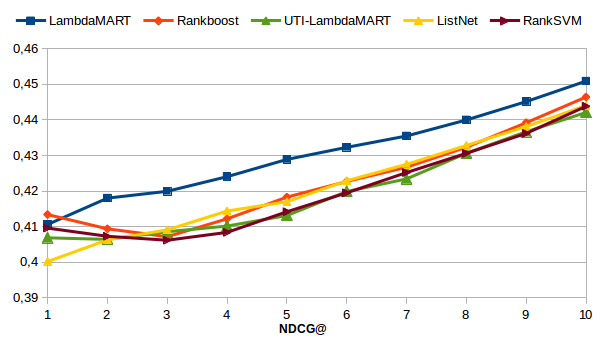
\includegraphics[width=10cm, height=5cm]{im_ndcg_baseline.png}

\caption{Comparison Results with NDCG@1 to NDCG@10 on LETOR}

\label{fig:ndcg10}

\end{center}

\end{figure}

While in LETOR there is almost no difference between UTI methods and other
learning methods, in practice search engines may contain
important features, not present in LETOR, but available at query processing time. For example, search engines can use the clicks performed by the users in the top results or personalized information collected from the user's history. For this reason, it is also important to analyze the performance of UTI-LambdaMART as a base ranker.

\begin{figure}[ht!]
\centering
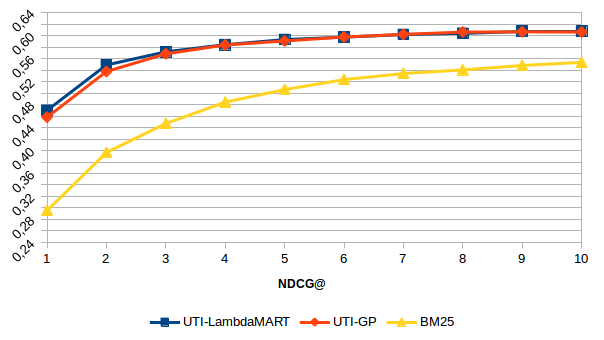
\includegraphics[width=10cm, height=5cm]{im_ndcg10leprefbm25.png}
\caption{LambdaMART results achieved when using BM25, UTI-LamdaMART and UTI-GP as base rankers}
\label{fig:bm25}
\end{figure}


Figure~\ref{fig:bm25} compares the
performance of BM25, UTI-GP, and UTI-LambdaMART when used as base rankers for \lambdamart.
We can see that both UTI-based models outperform BM25 as a base ranker. For example, on the top
2 results, we achieve value of NDCG of 0.55 when using
UTI-LambdaMART, while to achieve the same quality with BM25 we need to
take the 9 top results.

This result shows that UTI-LambdaMART can be effectively employed 
in practical web search scenarios as a base ranker.
First, as shown in Figure~\ref{fig:bm25}, it reduces the number of top results that must be processed by the top ranker. 
Second, it reduces the amount of features to be fetched and computed at query processing time, since UTI values represent information extracted from all features available at indexing times. In fact, the UTI values enconde 26 features available at indexing times in LETOR, and only the remaining 20 features would be fetched at query processing times.

\subsection{Reducing the Index Size}
\label{sec:compression}

A common approach for improving search engine time and space efficiency is to compress the inverted index~\cite{baezaribeiro2011modinforet}. A compressed index will take less storage space and thus require less I/O operations, generally yielding a gain in performance. In our proposal, we can exploit UTI-\lambdamart\ to achieve a much smaller index with low impact on its construction time. In addition, our approach will still allow the complementary application of standard compression methods, thus possibly yielding even greater gains.

Our proposal for index size reduction consists in, quite simply, truncating the decimal places in the UTI values generated. In Algorithm~\ref{alg:utilambda}, every time the function $Ft_n$ is evaluated, only the first $d$ decimal places are considered. A smaller value for $d$ means less bytes required for storage per UTI. Interestingly, even though this will limit the precision of the document score calculation, UTI-\lamdamart\ will still try to optimize the final ranking, thus minimizing the impact that this loss of information might have on the quality of the results, as we show in the following experiments.

\begin{figure}[ht!]
\centering
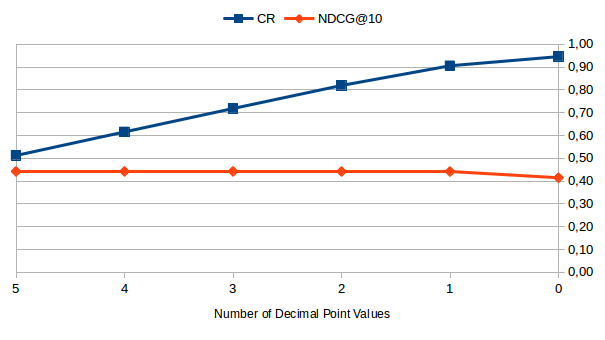
\includegraphics[width=10cm, height=5cm]{im_cr_ndcg_lambda.png}
\caption{Compression rate achieved by applying Elias-$\delta$ to the UTI values (varying the number of digits truncated from 0 to 5) produced by UTI-LambdaMART in the index and the NDCG@10 achieved when varying the number of truncated digits;}
\label{fig:crq}
\end{figure}

Figure~\ref{fig:crq} shows the compression rates achieved when varying the number of digits truncated in the UTI value, applying the technique to. Without loss of generality, in addition to our approach, we also compressed the truncated UTI values with the commonly used technique of \textit{Elias Delta codes}~\cite{elias1975universal}. To compute the compression rate, we assume that each original UTI value (i.e. non-truncated) would be represented as a 32 bit floating point number. 

As can be seen, there is indeed a trade-off between quality and compression rate as we vary the number of decimal point values truncated when transforming real values of UTI into integer values.
Nevertheless, results of truncating the UTI to only $1$ decimal digit yields only a reduction of 0.0004 in NDCG, while achieving a compression rate of about 83\%.
When truncating to zero digits, we see a clear negative impact in the NDCG values, indicating that the best tradeoff was achieved in fact when $d=1$.

\section{Conclusion}

We proposed the UTI-LambdaMART, a modified LambdaMART ranking algorithm, in order to generate UTI scores for each pair of query term and document at indexing time.

The experimental results indicate that UTI-LambdaMART produces quality results closer to the ones produced by UTI-GP, while significantly reduces the time required for learning the model. 
We also investigated two scenarios, the use of UTI-LambdaMART as the base ranker and using UTI-LambdaMART as top ranker. In the first, UTI values are able to produce high quality first cut rankings that are close to the final document order, reducing the amount of documents necessary to be inspected in the top ranker and resulting
in gains of performance when comparing to a system that adopts BM25 as the base ranker. In the second scenario, UTI-LambdaMART is directly applied as the top ranker, and we show that, even taking only features available at indexing times, it produces rankings with quality closer to learn to rank methods adopted at query processing times, but with the advantage of adopting a very simple ranking
strategy at query processing times.


Our future investigations are to know which results will be achieved when the UTI score is used as a feature in the learning process and applied to traditional L2R approaches. Finally, we plan to further evaluate the possible gains in query processing times generated by the use of   UTI-LambdaMART.

\label{conclusion}



\bibliographystyle{elsarticle-num}

% \bibliographystyle{elsarticle-harv}

% \bibliographystyle{elsarticle-num-names}

% \bibliographystyle{model1a-num-names}

% \bibliographystyle{model1b-num-names}

% \bibliographystyle{model1c-num-names}

% \bibliographystyle{model1-num-names}

% \bibliographystyle{model2-names}

% \bibliographystyle{model3a-num-names}

% \bibliographystyle{model3-num-names}

% \bibliographystyle{model4-names}

% \bibliographystyle{model5-names}

% \bibliographystyle{model6-num-names}


\bibliography{sample}


\end{document}

%%
%% End of file `elsarticle-template-num.tex'.
